% questions.tex —— 1977 年·内蒙古卷·理科 · 题目内容片段（无答案）
% 由 tools/generate_projects.py 依来源总账自 1977/1977_数学真题_内蒙古理_试题.md 生成，勿手改（改源 MD 后重跑）


\gkpart{数学试题解（理科）}

\begin{gktip}
\textbf{来源说明}：本题面依据固定源 PDF《内蒙古 1977 年高考数学试题解（理科）》第 1—4 页逐题转录，解答依据同一 PDF 第 1—6 页核对。固定源是题面与解答连续出现的扫描材料，而不是无答案试卷；题面完整性和源解答对应关系已逐页记录。正式题为第 1—6 题，末尾“附加题（20 分，不计入总分）”的两题不计入题量。
\end{gktip}

\begin{question}
\gkti{1}\textbf{（30 分）} 

\Needspace{5\baselineskip}
（1） 化简：

\nopagebreak[4]
\[
\sqrt{4-12a+9a^2}
\]

\Needspace{5\baselineskip}
（2） 计算：

\nopagebreak[4]
\[
\frac{(-27)^3\sqrt{\left(\frac1{16}\right)^{-\frac12}}}
{(-9)^0\left(\frac32\right)^7\left(\frac12\right)^{-5}}
\]

（3） 已知 $\lg2=0.3010$，$f(x)=\log_{\sqrt{10}}x$，求 $f(5)$。

\Needspace{5\baselineskip}
（4） 求函数

\nopagebreak[4]
\[
y=\frac{\sqrt{1-\frac23x}}{\sqrt[3]{3x-1}}
\]

的定义域。

\Needspace{5\baselineskip}
（5） 已知 $\cos\theta=0.6$，$270^\circ<\theta<360^\circ$，求

\nopagebreak[4]
\[
\left(\sin\frac\theta2-\cos\frac\theta2\right)^2
\]

的值。

\Needspace{5\baselineskip}
（6） 把点 $P$ 的极坐标

\nopagebreak[4]
\[
\left(-4,-\frac{4\pi}{3}\right)
\]

化成直角坐标。

\Needspace{0.4\textheight}
\end{question}
\begin{question}
\gkti{2}\textbf{（14 分）} 

（1） 已知：梯形 $ABCD$，$AD\parallel BC$，对角线 $AC$ 和 $BD$ 相交于 $E$，过 $E$ 作平行于底的直线，交 $AB$ 于 $M$，交 $CD$ 于 $N$。求证：$ME=EN$。
\nopagebreak[4]
\begin{center}% 1977 年内蒙古卷理科第 2(1) 题：梯形对角线与平行截线
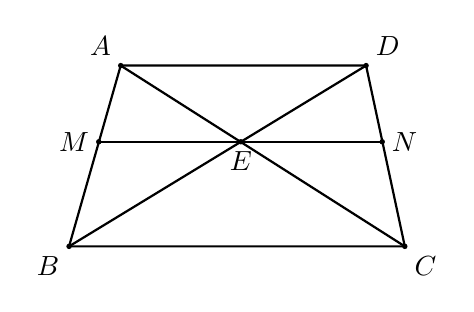
\begin{tikzpicture}[scale=0.82]
  \coordinate (A) at (0.8,2.8);
  \coordinate (D) at (4.6,2.8);
  \coordinate (B) at (0,0);
  \coordinate (C) at (5.2,0);
  \coordinate (E) at (2.66,1.62);
  \coordinate (M) at (0.46,1.62);
  \coordinate (N) at (4.85,1.62);
  \draw[thick] (A)--(D)--(C)--(B)--cycle;
  \draw[thick] (A)--(C);
  \draw[thick] (B)--(D);
  \draw[thick] (M)--(N);
  \fill (A) circle (1.2pt) node[above left] {$A$};
  \fill (D) circle (1.2pt) node[above right] {$D$};
  \fill (B) circle (1.2pt) node[below left] {$B$};
  \fill (C) circle (1.2pt) node[below right] {$C$};
  \fill (E) circle (1.2pt) node[below] {$E$};
  \fill (M) circle (1.2pt) node[left] {$M$};
  \fill (N) circle (1.2pt) node[right] {$N$};
\end{tikzpicture}
\end{center}
\nopagebreak[4]
（2） 圆台上底直径为 $12\ \mathrm{cm}$，下底直径为 $24\ \mathrm{cm}$，高为 $8\ \mathrm{cm}$，求圆台的全面积。（$\pi\approx3.14$，精确到 $0.1\ \mathrm{cm^2}$。）

\end{question}
\begin{question}
\gkti{3}\textbf{（12 分）} 红旗拖拉机厂今年元月份生产出一批甲、乙两种型号的拖拉机，其中生产乙型 16 台。从二月份起，甲型每月增产 10 台，而乙型按每月相同增长率逐步递增。又知二月份甲、乙两型拖拉机产量之比是 $3:2$，三月份甲、乙两型拖拉机产量之和是 65 台。求乙型拖拉机每月的增长率及甲型拖拉机元月份的产量。

\end{question}
\begin{question}
\gkti{4}\textbf{（14 分）} 已知：直线 $3x+y=5$ 及 $2x-3y+4=0$ 交于 $A$ 点。求：

（1） 过 $A$ 点且与 $y$ 轴垂直的直线方程；

（2） 过 $A$ 点且与圆 $x^2+y^2=1$ 相切的直线方程。

\Needspace{0.4\textheight}
\end{question}
\begin{question}
\gkti{5}\textbf{（15 分）} 甲、乙两船，甲船在某岛 $B$ 的正南方向 $A$ 处，$AB=10$ 海里，甲船自 $A$ 处以 $4$ 海里/小时的速度向正北方向航行；同时，乙船以 $6$ 海里/小时的速度自 $B$ 出发，向岛的北 $60^\circ$ 西方向驶去，问几分钟后两船相距最近？（精确到 1 分。）
\nopagebreak[4]
\begin{center}% 1977 年内蒙古卷理科第 5 题：两船航行示意图
\begin{tikzpicture}[scale=0.68]
  \coordinate (A) at (0,0);
  \coordinate (B) at (0,5.0);
  \coordinate (C) at (0,2.25);
  \coordinate (D) at (2.8,5.0);
  \draw[thick] (A)--(B);
  \draw[thick] (B)--(D);
  \draw[thick] (C)--(D);
  \draw[dashed] (C)--(B);
  \fill (A) circle (1.2pt) node[below left] {$A$};
  \fill (B) circle (1.2pt) node[left] {$B$};
  \fill (C) circle (1.2pt) node[left] {$C$};
  \fill (D) circle (1.2pt) node[right] {$D$};
  \node[right] at (0,3.65) {甲船};
  \node[above] at (1.35,5.0) {乙船};
  \node[right] at (0,2.25) {$4x$};
  \node[left] at (0,3.6) {$10-4x$};
  \node[above] at (1.4,5.0) {$6x$};
  \node at (1.0,4.1) {$60^\circ$};
\end{tikzpicture}
\end{center}
\nopagebreak[4]
\end{question}
\begin{question}
\gkti{6}\textbf{（15 分）} 

已知：在 $\triangle ABC$ 中，$a\text{、}b\text{、}c$ 是三个内角 $A\text{、}B\text{、}C$ 的对边，$\lg\sin A\text{、}\lg\sin B\text{、}\lg\sin C$ 成等差数列。

\Needspace{5\baselineskip}
（1） 求证：

\nopagebreak[4]
\[
\frac{\sin^2A}{\sin^2B}=\frac ac
\]

\Needspace{5\baselineskip}
（2） 又若方程

\nopagebreak[4]
\[
cx^2+2cx+a=0
\]

有相等的两个实根，求证：$\sin A=\sin B=\sin C$。

\begin{gktip}
\textbf{附加题（20 分，不计入总分）}
\end{gktip}

\Needspace{5\baselineskip}
\textbf{附加题 1．} 在 $\triangle ABC$ 中，求证：

\nopagebreak[4]
\[
\sin^2A+\sin^2B+\cos^2C+2\sin A\sin B\cos(A+B)=1
\]

\Needspace{5\baselineskip}
\textbf{附加题 2．} 已知：椭圆的中心点在原点，长轴和短轴都在坐标轴上，离心率 $e=0.8$，一条准线方程为

\nopagebreak[4]
\[
y=-\frac{25}{4}
\]

求内接于椭圆的最大矩形面积。

\end{question}